\documentclass[tikz,border=0pt]{standalone}
\usepackage{xcolor}
\usetikzlibrary{calc}
% Palette: Sam_Comm_final.png by eye, and the drones and raiders.
\definecolor{ink}{HTML}{3B2340}
\definecolor{sky}{HTML}{EFC46A}
\definecolor{skyhi}{HTML}{F5DA92}
\definecolor{skylow}{HTML}{E9B060}
\definecolor{cloud}{HTML}{F2D58A}
\definecolor{paper}{HTML}{FBEFD0}
\definecolor{cream}{HTML}{FFF6E0}
\definecolor{white}{HTML}{FFFFFF}
\definecolor{wallA}{HTML}{E88A73}
\definecolor{wallB}{HTML}{EE9F7E}
\definecolor{wallC}{HTML}{E47A7E}
\definecolor{wallD}{HTML}{F0B07E}
\definecolor{wallE}{HTML}{D9765F}
\definecolor{wallF}{HTML}{E99A8A}
\definecolor{greenA}{HTML}{8DBB7E}
\definecolor{greenB}{HTML}{6FA77A}
\definecolor{greenC}{HTML}{A9C97F}
\definecolor{greenD}{HTML}{5E9C6A}
\definecolor{greenE}{HTML}{4A8060}
\definecolor{sage}{HTML}{9DB98A}
\definecolor{sagedark}{HTML}{6F8F66}
\definecolor{sagelight}{HTML}{C2D6A6}
\definecolor{window}{HTML}{F6E7A0}
\definecolor{windark}{HTML}{8C5A64}
\definecolor{metal}{HTML}{8D9A93}
\definecolor{metaldark}{HTML}{5E6B66}
\definecolor{metallight}{HTML}{B9C4BC}
\definecolor{wood}{HTML}{B9835A}
\definecolor{wooddark}{HTML}{8C5A3C}
\definecolor{woodlight}{HTML}{D9A66F}
\definecolor{stone}{HTML}{E7C9A0}
\definecolor{stonedark}{HTML}{C9A47E}
\definecolor{concrete}{HTML}{D8C3A4}
\definecolor{concretedark}{HTML}{B8A084}
\definecolor{asphalt}{HTML}{8E7A86}
\definecolor{asphaltdark}{HTML}{6E5C68}
\definecolor{roadline}{HTML}{F6E7A0}
\definecolor{kerb}{HTML}{D8B48C}
\definecolor{red}{HTML}{E0483E}
\definecolor{redlight}{HTML}{F27A6A}
\definecolor{gold}{HTML}{FFB000}
\definecolor{goldlight}{HTML}{FFD54F}
\definecolor{teal}{HTML}{4FA3A0}
\definecolor{tealdark}{HTML}{3C8582}
\definecolor{magenta}{HTML}{FF2E88}
\definecolor{cyan}{HTML}{13CFE3}
\definecolor{violet}{HTML}{8A5BD6}
\definecolor{orange}{HTML}{F2803A}
\definecolor{pink}{HTML}{F48FB1}
\definecolor{glow}{HTML}{4FE6E0}
\definecolor{glowhi}{HTML}{C8FFF9}
\definecolor{hot}{HTML}{FF6A1A}
\definecolor{hothi}{HTML}{FFD07A}
\definecolor{armour}{HTML}{7E7A86}
\definecolor{armourdark}{HTML}{5A5466}
\definecolor{armourlight}{HTML}{A8A2B0}
\definecolor{wasp}{HTML}{E0A82E}
\definecolor{waspdark}{HTML}{B07E1A}
\definecolor{moth}{HTML}{F2E6C8}
\definecolor{mothdark}{HTML}{D2C09A}
\definecolor{hornet}{HTML}{3C8582}
\definecolor{hornetdark}{HTML}{2C6260}
\definecolor{warden}{HTML}{E47A7E}
\definecolor{wardendark}{HTML}{B85A62}
\definecolor{tick}{HTML}{8DBB7E}
\definecolor{tickdark}{HTML}{5E8A5A}
\definecolor{strider}{HTML}{D9765F}
\definecolor{striderdark}{HTML}{A8543F}
\definecolor{jacket}{HTML}{6FA77A}
\definecolor{jacketb}{HTML}{4FA3A0}
\definecolor{jacketc}{HTML}{E88A73}
\definecolor{jacketd}{HTML}{F0B07E}
\definecolor{skin}{HTML}{F2C49A}
\definecolor{skinb}{HTML}{C98C6A}
\definecolor{skinc}{HTML}{8C5A3C}
\definecolor{hair}{HTML}{3B2340}
\definecolor{goo}{HTML}{B6E35A}
\definecolor{goodark}{HTML}{7FB23A}
\newcommand{\Ink}{1.8pt}
\tikzset{inked/.style={draw=ink, line width=\Ink, line join=round, line cap=round}}
\begin{document}
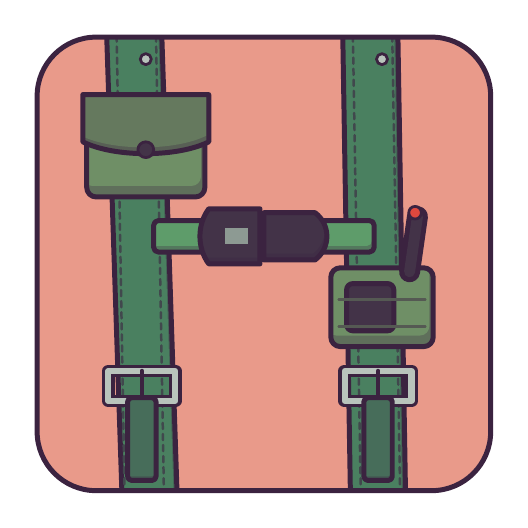
\begin{tikzpicture}
\clip (0,0) rectangle (6,6);
\fill[wallF] [rounded corners=0.75cm] (0.12,0.12) rectangle (5.88,5.88);
\begin{scope}\clip [rounded corners=0.75cm] (0.12,0.12) rectangle (5.88,5.88);
\begin{scope}\clip (1,6) -- (1.7,6) -- (1.9,0) -- (1.2,0) -- cycle;
\fill[greenE!70!ink] (1,6) -- (1.7,6) -- (1.9,0) -- (1.2,0) -- cycle;
\fill[greenE, shift={(-0.049,0.14)}] (1,6) -- (1.7,6) -- (1.9,0) -- (1.2,0) -- cycle;
\end{scope}
\draw[inked] (1,6) -- (1.7,6) -- (1.9,0) -- (1.2,0) -- cycle;
\draw[greenE!40!ink, line width=0.9pt, line cap=round, dash pattern=on 2.2pt off 1.8pt] (1.13,5.9) -- (1.23,0.1);
\draw[greenE!40!ink, line width=0.9pt, line cap=round, dash pattern=on 2.2pt off 1.8pt] (1.63,5.9) -- (1.73,0.1);
\begin{scope}\clip (4,6) -- (4.7,6) -- (4.8,0) -- (4.1,0) -- cycle;
\fill[greenE!70!ink] (4,6) -- (4.7,6) -- (4.8,0) -- (4.1,0) -- cycle;
\fill[greenE, shift={(-0.049,0.14)}] (4,6) -- (4.7,6) -- (4.8,0) -- (4.1,0) -- cycle;
\end{scope}
\draw[inked] (4,6) -- (4.7,6) -- (4.8,0) -- (4.1,0) -- cycle;
\draw[greenE!40!ink, line width=0.9pt, line cap=round, dash pattern=on 2.2pt off 1.8pt] (4.13,5.9) -- (4.23,0.1);
\draw[greenE!40!ink, line width=0.9pt, line cap=round, dash pattern=on 2.2pt off 1.8pt] (4.63,5.9) -- (4.73,0.1);
\begin{scope}\clip[rounded corners=0.06cm] (1.6,3.15) rectangle (4.4,3.55);
\fill[greenD!70!ink,rounded corners=0.06cm] (1.6,3.15) rectangle (4.4,3.55);
\fill[greenD,rounded corners=0.06cm, shift={(-0.028,0.08)}] (1.6,3.15) rectangle (4.4,3.55);
\end{scope}
\draw[inked,rounded corners=0.06cm] (1.6,3.15) rectangle (4.4,3.55);
\begin{scope}\clip (2.3,3.0) -- (2.95,3.0) -- (2.95,3.7) -- (2.3,3.7) .. controls (2.15,3.5) and (2.15,3.2) .. (2.3,3.0) -- cycle;
\fill[ink!78!metaldark!70!ink] (2.3,3.0) -- (2.95,3.0) -- (2.95,3.7) -- (2.3,3.7) .. controls (2.15,3.5) and (2.15,3.2) .. (2.3,3.0) -- cycle;
\fill[ink!78!metaldark, shift={(-0.028,0.08)}] (2.3,3.0) -- (2.95,3.0) -- (2.95,3.7) -- (2.3,3.7) .. controls (2.15,3.5) and (2.15,3.2) .. (2.3,3.0) -- cycle;
\end{scope}
\draw[inked] (2.3,3.0) -- (2.95,3.0) -- (2.95,3.7) -- (2.3,3.7) .. controls (2.15,3.5) and (2.15,3.2) .. (2.3,3.0) -- cycle;
\begin{scope}\clip (3.0,3.05) -- (3.65,3.05) .. controls (3.85,3.2) and (3.85,3.5) .. (3.65,3.65) -- (3.0,3.65) -- cycle;
\fill[ink!78!metaldark!70!ink] (3.0,3.05) -- (3.65,3.05) .. controls (3.85,3.2) and (3.85,3.5) .. (3.65,3.65) -- (3.0,3.65) -- cycle;
\fill[ink!78!metaldark, shift={(-0.028,0.08)}] (3.0,3.05) -- (3.65,3.05) .. controls (3.85,3.2) and (3.85,3.5) .. (3.65,3.65) -- (3.0,3.65) -- cycle;
\end{scope}
\draw[inked] (3.0,3.05) -- (3.65,3.05) .. controls (3.85,3.2) and (3.85,3.5) .. (3.65,3.65) -- (3.0,3.65) -- cycle;
\fill[metal] (2.5,3.25) rectangle (2.8,3.45);
\draw[ink, line width=4.6pt, line join=round] (1.025,1.26) -- (1.875,1.26) -- (1.875,1.64) -- (1.025,1.64) -- cycle;
\draw[metallight, line width=2.2pt, line join=round] (1.025,1.26) -- (1.875,1.26) -- (1.875,1.64) -- (1.025,1.64) -- cycle;
\draw[ink, line width=1.6pt, line cap=round] (1.45,1.26) -- (1.45,1.64);
\begin{scope}\clip[rounded corners=0.05cm] (1.27,0.25) rectangle (1.63,1.3);
\fill[greenE!80!ink!70!ink,rounded corners=0.05cm] (1.27,0.25) rectangle (1.63,1.3);
\fill[greenE!80!ink,rounded corners=0.05cm, shift={(-0.017,0.05)}] (1.27,0.25) rectangle (1.63,1.3);
\end{scope}
\draw[inked,rounded corners=0.05cm] (1.27,0.25) rectangle (1.63,1.3);
\draw[ink, line width=4.6pt, line join=round] (4.025,1.26) -- (4.875,1.26) -- (4.875,1.64) -- (4.025,1.64) -- cycle;
\draw[metallight, line width=2.2pt, line join=round] (4.025,1.26) -- (4.875,1.26) -- (4.875,1.64) -- (4.025,1.64) -- cycle;
\draw[ink, line width=1.6pt, line cap=round] (4.45,1.26) -- (4.45,1.64);
\begin{scope}\clip[rounded corners=0.05cm] (4.27,0.25) rectangle (4.63,1.3);
\fill[greenE!80!ink!70!ink,rounded corners=0.05cm] (4.27,0.25) rectangle (4.63,1.3);
\fill[greenE!80!ink,rounded corners=0.05cm, shift={(-0.017,0.05)}] (4.27,0.25) rectangle (4.63,1.3);
\end{scope}
\draw[inked,rounded corners=0.05cm] (4.27,0.25) rectangle (4.63,1.3);
\begin{scope}\clip[rounded corners=0.12cm] (0.75,3.85) rectangle (2.25,5.1);
\fill[sagedark!70!ink,rounded corners=0.12cm] (0.75,3.85) rectangle (2.25,5.1);
\fill[sagedark,rounded corners=0.12cm, shift={(-0.049,0.14)}] (0.75,3.85) rectangle (2.25,5.1);
\end{scope}
\draw[inked,rounded corners=0.12cm] (0.75,3.85) rectangle (2.25,5.1);
\begin{scope}\clip (0.7,5.15) -- (2.3,5.15) -- (2.3,4.55) .. controls (1.9,4.35) and (1.1,4.35) .. (0.7,4.55) -- cycle;
\fill[sagedark!80!ink!70!ink] (0.7,5.15) -- (2.3,5.15) -- (2.3,4.55) .. controls (1.9,4.35) and (1.1,4.35) .. (0.7,4.55) -- cycle;
\fill[sagedark!80!ink, shift={(-0.028,0.08)}] (0.7,5.15) -- (2.3,5.15) -- (2.3,4.55) .. controls (1.9,4.35) and (1.1,4.35) .. (0.7,4.55) -- cycle;
\end{scope}
\draw[inked] (0.7,5.15) -- (2.3,5.15) -- (2.3,4.55) .. controls (1.9,4.35) and (1.1,4.35) .. (0.7,4.55) -- cycle;
\filldraw[inked,fill=ink!78!metaldark,line width=1.0pt] (1.5,4.45) circle (0.1);
\begin{scope}\clip[rounded corners=0.12cm] (3.85,1.95) rectangle (5.15,2.95);
\fill[sagedark!70!ink,rounded corners=0.12cm] (3.85,1.95) rectangle (5.15,2.95);
\fill[sagedark,rounded corners=0.12cm, shift={(-0.049,0.14)}] (3.85,1.95) rectangle (5.15,2.95);
\end{scope}
\draw[inked,rounded corners=0.12cm] (3.85,1.95) rectangle (5.15,2.95);
\draw[ink, line width=7.583pt, line cap=round, line join=round] plot[smooth, tension=0.6] coordinates {(4.85,2.9) (4.95,3.6)};
\draw[ink!78!metaldark, line width=3.983pt, line cap=round, line join=round] plot[smooth, tension=0.6] coordinates {(4.85,2.9) (4.95,3.6)};
\begin{scope}\clip[rounded corners=0.08cm] (4.05,2.15) rectangle (4.65,2.75);
\fill[ink!78!metaldark!70!ink,rounded corners=0.08cm] (4.05,2.15) rectangle (4.65,2.75);
\fill[ink!78!metaldark,rounded corners=0.08cm, shift={(-0.017,0.05)}] (4.05,2.15) rectangle (4.65,2.75);
\end{scope}
\draw[inked,rounded corners=0.08cm] (4.05,2.15) rectangle (4.65,2.75);
\filldraw[inked,fill=red,line width=1.0pt] (4.92,3.65) circle (0.08);
\draw[sagedark!50!ink, line width=1pt, line cap=round] (3.95,2.2) -- (5.05,2.2);
\draw[sagedark!50!ink, line width=1pt, line cap=round] (3.95,2.55) -- (5.05,2.55);
\filldraw[inked,fill=metallight,line width=1.0pt] (1.5,5.6) circle (0.07);
\filldraw[inked,fill=metallight,line width=1.0pt] (4.5,5.6) circle (0.07);
\end{scope}
\draw[inked] [rounded corners=0.75cm] (0.12,0.12) rectangle (5.88,5.88);
\end{tikzpicture}
\end{document}
